%cd '/mnt/ExtraDrive1/Work/desktop_data/ActiveBooks/GeostatDale/Rcode/Chapter11/Section spglm'
% bibtex section_spglm

% ------------------------------------------------------------------------------
%
% PREAMBLE
%
% ------------------------------------------------------------------------------

\documentclass[12pt, titlepage]{article}


\usepackage{graphicx, amsmath, amssymb, natbib, setspace, sectsty, verbatim, 
		mathrsfs, float}
\usepackage{MnSymbol}
\usepackage{multirow}
\usepackage{bm}
\usepackage[usenames, dvipsnames]{color}
\bibpunct{(}{)}{;}{a}{}{,}
\setlength{\parindent}{3em}
%\parskip = 1.5ex
%\linespread{1.3}
%\onehalfspacing

\pdfpagewidth 8.5in
\pdfpageheight 11in
\setlength{\oddsidemargin}{0.0in} \setlength{\textwidth}{6.5in}
\setlength{\topmargin}{0.15in} \setlength{\textheight}{8.5in}
\setlength{\headheight}{0.0in} \setlength{\headsep}{0.0in}

\usepackage{/mnt/ExtraDrive1/Work/shTex/mymacros}


% ------------------------------------------------------------------------------
%
% BEGIN DOCUMENT
%
% ------------------------------------------------------------------------------

\begin{document}

\setcounter{equation}{0}
\renewcommand{\theequation}{12.\arabic{equation}}


% ------------------------------------------------------------------------------
%
%                    Section 8.8.1
%                    Seal trend data
%
% ------------------------------------------------------------------------------

{\Large \flushleft \textbf{12.x Spatial Generalized Linear Models}}

\vspace{.3cm}

Many types of data are binary, counts, or positive continuous.  Early attempts to model such data relied on transformations to ``near normal'' so that classical linear model methods could be used.  For example, a square root transformation was often used for count data.  However, \citet{NelderEtAl1972GeneralizedLinearModels370} introduced a natural extension to linear models using parameteric distributions such as the Poisson for counts, the Bernoulli for binary data, etc., called the generalized linear model \citep[GLM,][]{McCullaghEtAl1989GeneralizedLinearModels}, which have become very popular and generally preferred to data transformations.  A natural extension of GLMs by allowing latent random effects in the linear mixed model, to create a class of generalized linear mixed model \citep[GLMM,][]{breslow_approximate_1993}.  The latent random effects are generally assumed to be independent and identically distributed from normal distribution.  However, it is also possible to for the latent random effects to be spatially autocorrelated, leading to the spatial generalized linear model \citep[SGLM,][]{GotwayEtAl1997GeneralizedLinearModel157, DiggleEtAl1998ModelbasedGeostatisticsDisc299}, which we review here.

Historically, for areal data, such as the models in Chapter 7, there are equivalent models for discrete data, such as those that are binary or counts.  These have been termed the autologistic, auto-Poisson models, autobinomial, and auto negative binomial, with obvious connections to their nonspatial distributions \citep{Besag1974SpatialInteractionStatistical192, Cressie1993StatisticsSpatialData}.  These models have not been very popular, as the conditional specification does not always lead to a recognizable likelihood, or, indeed, as for the auto-Poisson, that likelihood may not have a closed form under positive autocorrelation.  We will not discuss these models further.

Another class of models are based on a hierarchical constuction, where the mean of any of the distributions in GLMs is allowed to vary by using spatial random effects in the mean structure.  Here, there are three broad methods of analysis.  The most obvious method is to take a Bayesian approach and compute the posterior distribution of all latent spatial variables and parameters.  This has been extremely popular beginning with disease-mapping \citep{clayton_empirical_1987} and the introduction of the \texttt{WinBUGS} software \citep{lunn_winbugs-bayesian_2000}. 

Another approach is the penalized quasi-likelihood models \citep{breslow_approximate_1993, WolfingerEtAl1993GeneralizedLinearMixed233}.  These models have been implemented in popular software such as the \texttt{glmmPQL} function in the \texttt{MASS} package in \texttt{R} and the \texttt{GLIMMIX} package in \texttt{SAS}.

A third approach is to take a likelihood approach and attempt to estimate covariance parameter, and perhaps fixed effects simultaneously, while integrating out over all spatial random effects.   This can be done using Markov chain Monte Carlo methods \citep[e.g.,][]{christensen_monte_2004} or more directly using a Laplace approximation \citep[e.g.,][]{evangelou_estimation_2011, bonat_practical_2016}.  Here, we will follow \citet{bonat_practical_2016}, and improve their methods.




% ------------------------------------------------------------------------------
% ------------------------------------------------------------------------------
% ------------------------------------------------------------------------------
%                  12.x.1 Spatially structured dependence
% ------------------------------------------------------------------------------
% ------------------------------------------------------------------------------
% ------------------------------------------------------------------------------

{\large \flushleft \textbf{12.x.1 Spatially structured dependence}}

A very general way to create spatially structured dependence for GLMMs is through a hierarchical construction.  We will use the notation $[\mathbf{y}|\boldsymbol{\xi}]$ to denote any probability density function of the vector of random variables $\mathbf{y}$ conditional on a vector of parameters, or other fixed variables, $\boldsymbol{\xi}$. We can have a joint distribution on the left side of the conditional bar, and multiple parameter and fixed value vectors on the right, e.g., $[\mathbf{y}_{1},\mathbf{y}_{2}, \ldots, \mathbf{y}_{k} | \boldsymbol{\xi}_{1}, \boldsymbol{\xi}_{2}, \ldots, \boldsymbol{\xi}_{k}]$. For example, let $[\mathbf{y}|\boldsymbol{\xi}]$ be the product of independent Poisson distributions with mean parameters contained in the vector $\boldsymbol{\xi}$.  For the hierarchical construction of a SGLM, we condition on spatially-autocorrelated random effects $\mathbf{w}$, thus $[\mathbf{y}|\mathbf{w}]$, where $\mathbf{w}$ is generally considered to have multivariate normal distribution, which can be denoted $[\mathbf{w}|\boldsymbol{\theta}]$, where the vector $\boldsymbol{\theta}$ contains covariance parameters.  For example, $\boldsymbol{\theta}$ often contains the partial sill, range, and nugget effect for geostatistical models (Chapter 6), or may contain the variance and autocorrelation parameters from Chapter 7.  Hence, the joint distribution of the data $\mathbf{y}$ and the latent spatial random effects $\mathbf{w}$ is $[\mathbf{y},\mathbf{w}|\boldsymbol{\theta}] = [\mathbf{y}|\mathbf{w}][\mathbf{w}|\boldsymbol{\theta}]$.  

The model for the data $\mathbf{y}$ can have more parameters than just the mean, in which case we write it $[\mathbf{y}|\boldsymbol{\mu},\boldsymbol{\phi}]$, where it is parameterized so that $\textrm{E}(\mathbf{y}) = \boldsymbol{\mu}$.  If our linear model is $\boldsymbol{\eta}$, then generalized linear models establish a link function between $\boldsymbol{\mu}$ and $\boldsymbol{\eta}$, which we denote as $g(\boldsymbol{\mu}) = \mathbf{w}$, where $g(\cdot)$ is called the link function.  For the Poisson example, $g(\cdot)$ is often the log function.  Link functions are monotonic so that $g^{-1}(\cdot)$ is one-to-one with $g(\cdot)$.  The log link makes sense for the Poisson example because, recall that the mean of a Poisson distribution must be postive, and $g^{-1}(\cdot)$ is the exponential function, and hence $\boldsymbol{\mu} = g^{-1}(\mathbf{w})$ is always positive and $\mathbf{w}$ is unconstrained on the real line, as it must be for a multivariate normal distribution. For an example with extra parameters for $\mathbf{y}$, consider the negative binomial distribution, which can be parameterized with a mean, and an extra parameter that allows for overdispersion, which we would write as $[\mathbf{y}|\boldsymbol{\mu},\phi]$, where $\phi$ is the overdispersion parameter.  

Now, let us write
$$
\mathbf{w} = \mathbf{X}\boldsymbol{\beta} + \mathbf{e},
$$
where this model is the same one defined in (1.1), where $\var(\mathbf{e}) = \boldsymbol{\Sigma}_{\boldsymbol{\theta}}$, and we use the subscript to show the dependence of $\boldsymbol{\Sigma}$ on $\boldsymbol{\theta}$.  Thus, we use the notation $[\mathbf{w}|\mathbf{X},\boldsymbol{\beta},\boldsymbol{\theta}]$ to indicate the probability density function $N(\mathbf{X}\boldsymbol{\beta},\boldsymbol{\Sigma}_{\boldsymbol{\theta}})$.  Then, a very general model can be constructed hierarchically as,
\begin{equation} \label{eq:hsglm}
[\mathbf{y},\mathbf{w}|\boldsymbol{\phi},\boldsymbol{\beta},\boldsymbol{\theta},\mathbf{X}] = [\mathbf{y}|\mathbf{w},\boldsymbol{\phi}][\mathbf{w}|\boldsymbol{\beta},\boldsymbol{\theta},\mathbf{X}].
\end{equation}
As a concrete example, suppose that $[\mathbf{y}|\mathbf{w}]$ is Poisson, and $[\mathbf{w}|\boldsymbol{\beta},\boldsymbol{\theta},\mathbf{X}]$ is multivariate normal, then the joint likelihood is
$$
[\mathbf{y},\mathbf{w}|\boldsymbol{\phi},\boldsymbol{\beta},\boldsymbol{\theta},\mathbf{X}] = \left(\prod_{i=1}^{n}\frac{\exp(w_{i})^{y_{i}}\exp(-\exp(w_i))}{y_{i}!}\right)\frac{\exp-[(\mathbf{w} - \mathbf{X}\boldsymbol{\beta})^{T}\boldsymbol{\Sigma_{\boldsymbol{\theta}}}^{-1}(\mathbf{w} - \mathbf{X}\boldsymbol{\beta})]}{(2\pi)^{n/2}|\boldsymbol{\Sigma_{\boldsymbol{\theta}}}|^{1/2}},
$$
and note the use of $\mu_{i} = g^{-1}(w_{i}) = \exp(w_{i})$.

The joint distribution \ref{eq:hsglm} forms the basis for inference, with popular choices given by
\begin{itemize}
\item putting prior distributions on $\boldsymbol{\phi}$, $\boldsymbol{\beta}$, and $\boldsymbol{\theta}$ and computing, or sampling from, the joint posterior distribution $[\mathbf{w},\boldsymbol{\phi},\boldsymbol{\beta},\boldsymbol{\theta}|\mathbf{y},\mathbf{X}]$ using any of a variety of Bayesian methods, or 
\item approximating \eqref{eq:hsglm} with a quasi-likehood and using iterative fitting algorithms for $\mathbf{w},\boldsymbol{\phi},\boldsymbol{\beta},\boldsymbol{\theta}$, or
\item integrating over $\mathbf{w}$ using a Laplace approximation, and integrating over $\boldsymbol{\beta}$ as in REML, and use maximum likelihood to estimate $\boldsymbol{\phi},\boldsymbol{\theta}$ marginally, followed by GLS estimation of $\boldsymbol{\beta}$ and prediction for $\mathbf{w}$.
\end{itemize}

Below, we will give more details on the Laplace approximation and the marginal maximum likelihood approach.

% ------------------------------------------------------------------------------
% ------------------------------------------------------------------------------
% ------------------------------------------------------------------------------
%               12.x.2 Exploratory spatial data analysis
% ------------------------------------------------------------------------------
% ------------------------------------------------------------------------------
% ------------------------------------------------------------------------------

{\large \flushleft \textbf{12.x.2 Exploratory spatial data analysis}}

la te da

% ------------------------------------------------------------------------------
% ------------------------------------------------------------------------------
% ------------------------------------------------------------------------------
%               12.x.3 Parametric models for the mean structure
% ------------------------------------------------------------------------------
% ------------------------------------------------------------------------------
% ------------------------------------------------------------------------------


{\large \flushleft \textbf{12.x.3 Parametric models for the mean structure}}

 la te da

% ------------------------------------------------------------------------------
% ------------------------------------------------------------------------------
% ------------------------------------------------------------------------------
%           12.x.4 Parametric models for the covariance structure
% ------------------------------------------------------------------------------
% ------------------------------------------------------------------------------
% ------------------------------------------------------------------------------

{\large \flushleft \textbf{12.x.4 Parametric models for the covariance structure}}

la te da

% ------------------------------------------------------------------------------
% ------------------------------------------------------------------------------
% ------------------------------------------------------------------------------
%           Marginal Maximum Likelihood Estimation
% ------------------------------------------------------------------------------
% ------------------------------------------------------------------------------
% ------------------------------------------------------------------------------

\vspace{.5cm}
{\large \flushleft \textbf{12.x.5 Marginal MLE for Covariance Parameters}}
\vspace{.5cm}

We would like to marginalize the distribution $[\mathbf{w}, \mathbf{y}|\boldsymbol{\phi},\boldsymbol{\beta},\boldsymbol{\theta}] = [\mathbf{y}|\mathbf{w},\boldsymbol{\phi}][\mathbf{w}|\boldsymbol{\beta},\boldsymbol{\theta}]$ over both $\mathbf{w}$ and $\boldsymbol{\beta}$ to obtain a distribution of the only the data and variance/covariance parameters,
$$
	[\mathbf{y}|\boldsymbol{\phi},\boldsymbol{\theta}] = \int_\mathbf{w} \int_{\boldsymbol{\beta}} [\mathbf{w}, \mathbf{y}|\boldsymbol{\phi},\boldsymbol{\beta},\boldsymbol{\theta}] d\boldsymbol{\beta} d\mathbf{w} =
		\int_\mathbf{w}  [\by|\mathbf{w},\boldsymbol{\phi}] \int_{\boldsymbol{\beta}} [\mathbf{w}|\boldsymbol{\beta},\boldsymbol{\theta}] d\boldsymbol{\beta} d\mathbf{w}.
$$
When $[\mathbf{w}|\boldsymbol{\beta},\boldsymbol{\theta}]$ is Gaussian, $\int_{\boldsymbol{\beta}} [\mathbf{w}|\boldsymbol{\beta},\boldsymbol{\theta}] d\boldsymbol{\beta}$ is the likelihood for restricted maximum likelihood estimation (REML) (see Exercise 8.4),
$$
[\mathbf{w}|\boldsymbol{\theta}] \equiv \int_{\boldsymbol{\beta}} [\mathbf{w}|\boldsymbol{\beta},\boldsymbol{\theta}] d\boldsymbol{\beta} = 
\frac{1}{C_n}\exp[(\mathbf{w} - \mathbf{X}\hat{\boldsymbol{\beta}})^{T}\boldsymbol{\Sigma}_{\boldsymbol{\theta}}^{-1}(\mathbf{w} - \mathbf{X}\hat{\boldsymbol{\beta}})],
$$
where $C_n = \sqrt{2\pi^N|\boldsymbol{\Sigma}_{\boldsymbol{\theta}}||\mathbf{X}^{T}\boldsymbol{\Sigma}_{\boldsymbol{\theta}}^{-1}\mathbf{X}|}$ and 
$\hat{\boldsymbol{\beta}} = (\mathbf{X}^{T}\boldsymbol{\Sigma}_{\boldsymbol{\theta}}^{-1}\mathbf{X})^{-1}\mathbf{X}^{T}\boldsymbol{\Sigma}_{\boldsymbol{\theta}}^{-1}\mathbf{w},$
and so we only need,
$$
	[\mathbf{y}| \boldsymbol{\phi},\boldsymbol{\theta}] = \int_\mathbf{w}  [\mathbf{y}|\mathbf{w},\boldsymbol{\phi}][\mathbf{w}|\boldsymbol{\theta}]d\mathbf{w}.
$$
Let us denote $\ell(\mathbf{w};\mathbf{y},\boldsymbol{\phi},\boldsymbol{\theta}) = \log([\mathbf{y}|\mathbf{w},\boldsymbol{\phi}][\mathbf{w}|\boldsymbol{\theta}])$, and consider $\int e^{\ell(\mathbf{w};\mathbf{y},\boldsymbol{\phi},\boldsymbol{\theta})} d\mathbf{w}$. Let $\mathbf{g}$ be the gradient vector with $i$th element
$$
g_{i} = \frac{\partial \ell(\mathbf{w};\mathbf{y},\boldsymbol{\phi},\boldsymbol{\theta})}{\partial w_i},
$$
and let $\mathbf{H}$ be the Hessian matrix with $i,j$th element,
$$
H_{i,j} = \frac{\partial^2 \ell(\mathbf{w};\mathbf{y},\boldsymbol{\phi},\boldsymbol{\theta})}{\partial w_i\partial w_j}.
$$
Using the multivariate Taylor series expansion around some point $\mathbf{a}$,
$$
\int_\mathbf{w} e^{\ell(\mathbf{w};\mathbf{y},\boldsymbol{\phi},\boldsymbol{\theta})} d\mathbf{w} \approx \int_\mathbf{w} e^{\ell(\mathbf{a};\mathbf{y},\boldsymbol{\phi},\boldsymbol{\theta}) + \mathbf{g}^{T}(\mathbf{w} -\mathbf{a}) + 1/2(\mathbf{w} - \mathbf{a})^{T}\mathbf{H}(\mathbf{w} - \mathbf{a})} d\mathbf{w}.
$$
Now, if $\mathbf{a}$ is a value for $\ell(\mathbf{a};\mathbf{y},\boldsymbol{\phi},\boldsymbol{\theta})$ such that $\mathbf{g} = \mathbf{0}$, then
$$
\int_\mathbf{w} e^{\ell(\mathbf{w};\mathbf{y},\boldsymbol{\phi},\boldsymbol{\theta})} d\mathbf{w} \approx e^{\ell(\mathbf{a};\mathbf{y},\boldsymbol{\phi},\boldsymbol{\theta})} \int_\bw e^{ -  
	1/2(\mathbf{w} - \mathbf{a})^{T}(-\mathbf{H})(\mathbf{w} - \mathbf{a})} d\mathbf{w}.
$$
Let $\mathbf{H}_\mathbf{a}$ indicate $\mathbf{H}$ evaluated at $\mathbf{a}$. We know from the normalizing constant of a multivariate Gaussian distribution that 
$$
\int_\bw e^{-1/2(\mathbf{w} - \mathbf{a})^{T}(-\mathbf{H}_{\mathbf{a}})(\mathbf{w} - \mathbf{a})} d\mathbf{w} = (2\pi)^{N/2}|-\mathbf{H}^{-1}_\mathbf{a}|^{1/2},
$$
so
\[
\int_\mathbf{w} e^{\ell(\mathbf{w};\mathbf{y},\boldsymbol{\phi},\boldsymbol{\theta})} d\mathbf{w} \approx e^{\ell(\mathbf{a};\mathbf{y},\boldsymbol{\phi},\boldsymbol{\theta})} (2\pi)^{N/2}|-\mathbf{H}_\mathbf{a}|^{-1/2} = [\mathbf{y}|\mathbf{a},\boldsymbol{\phi}][\mathbf{a}|\boldsymbol{\theta}](2\pi)^{N/2}|-\mathbf{H}_\mathbf{a}|^{-1/2}.
\]
A marginal maximum likelihood estimator for $\boldsymbol{\phi}, \boldsymbol{\theta}$, given $\mathbf{a}$, is
\begin{equation} \label{eq:m2LLmargMLE}
\{\hat{\boldsymbol{\phi}}, \hat{\boldsymbol{\theta}} \} = \underset{\boldsymbol{\phi},\boldsymbol{\theta}}{\arg\max} \left[ \log[\mathbf{y}|\mathbf{a},\mathbf{\phi}] +
	\log[\mathbf{a}|\mathbf{\theta}] - (1/2)\log(|-\mathbf{H}_\mathbf{a}(\boldsymbol{\phi},\boldsymbol{\theta})|) \right]
\end{equation}
where we drop terms that do not contain $\boldsymbol{\phi}$ or $\boldsymbol{\theta}$ and also show the dependence of $\mathbf{H}_\mathbf{a}$ on $\boldsymbol{\phi}$ and $\boldsymbol{\theta}$.  The result \eqref{eq:m2LLmargMLE} depends on finding $\mathbf{a}$ so that $\mathbf{g} = \mathbf{0}$.  To acheive this, we use Newton-Raphson, conditional on $\boldsymbol{\phi}$ and $\boldsymbol{\theta}$, which we describe next.

Assuming conditional independence of $\mathbf{y}$ on $\mathbf{w}$,
\begin{equation} \label{eq:ll_plus_C}
\log([\mathbf{y}|\mathbf{w},\boldsymbol{\phi}][\mathbf{w}|\boldsymbol{\theta}]) = \sum_{i = 1}^N \log[y_i|w_i,\boldsymbol{\phi}] - \frac{1}{2}(\mathbf{w} - \mathbf{X}\hat{\boldsymbol{\beta}})^{T}\boldsymbol{\Sigma}_{\boldsymbol{\theta}}^{-1}(\mathbf{w} - \mathbf{X}\hat{\boldsymbol{\beta}}) + C,
\end{equation}
where $C$ are terms that do not contain $\mathbf{w}$. Let $\mathbf{d}$ be the vector with $i$th component,
$$
d_{i} \equiv \frac{\partial\log[y_i|w_i,\boldsymbol{\phi}]}{\partial w_i},
$$
and
$$
\frac{\partial [-\frac{1}{2}(\mathbf{w} - \mathbf{X}\hat{\boldsymbol{\beta}})^{T}\boldsymbol{\Sigma}_{\boldsymbol{\theta}}^{-1}(\mathbf{w} - \mathbf{X}\hat{\boldsymbol{\beta}})]}{\partial \mathbf{w}} = -\boldsymbol{\Sigma}_{\boldsymbol{\theta}}^{-1}\mathbf{w} + \boldsymbol{\Sigma}_{\boldsymbol{\theta}}^{-1}\boldsymbol{X}\hat{\boldsymbol{\beta}},
$$
so the gradient of \eqref{eq:ll_plus_C} is
$$
\mathbf{g} = \mathbf{d} - \boldsymbol{\Sigma}_{\boldsymbol{\theta}}^{-1}\mathbf{w} + \boldsymbol{\Sigma}_{\boldsymbol{\theta}}^{-1}\mathbf{X}\hat{\boldsymbol{\beta}} = \mathbf{d} - \mathbf{P}_{\boldsymbol{\theta}}\mathbf{w},
$$
where $\mathbf{P}_{\boldsymbol{\theta}}$ was defined in (8.2). For the Hessian, let $\mathbf{D}$ be a diagonal matrix with $i$th component,
$$
D_{i,i} \equiv \frac{\partial^2\log[y_i|w_i,\boldsymbol{\phi}]}{\partial w_i^2},
$$
where all off-diagonal elements are zero because all second partials are 0 when $i \neq j$ due to conditional independence. A table of $\mathbf{d}_{i}$ and $\mathbf{D}_{i,i}$ for a few common distributions and link functions is given in Table~\ref{tab:dDlinkDist}.
\begin{table}[H] 
	\caption{Distributions, inverse link functions, and first and second partial derivative with respect to $w_{i}$ for the data model part of the loglikelihood.  \label{tab:dDlinkDist}}
\begin{center}
\begin{tabular}{|c|ccc|}
\hline
\hline
Distribution & $\mu = g^{-1}(\eta)$ & $\mathbf{d}_{i}$ & $\mathbf{D}_{i,i}$ \\
\hline
Binomial & $\mu =\frac{\exp(\eta)}{1+\exp(\eta)}$ & $y_{i} - \frac{n_{i}\exp(w_{i})}{1+\exp(w_{i})}$ & $- \frac{n_{i}\exp(w_{i})}{(1+\exp(w_{i}))^{2}}$ \\ 
Poisson & $\mu = \exp(\eta)$ & $y_{i} - \exp(w_{i})$ & $- \exp(w_{i})$ \\ 
Negative Binomial & $\mu = \exp(\eta)$ &  $
\frac{\phi(y_{i} - e^{w_{i}})}{\phi + e^{w_{i}}}$ & $-\frac{\phi e^{w_{i}}(\phi + y_{i})}{(\phi + e^{w_{i}})^{2}}$ \\ 
\hline
\hline
\end{tabular}
\end{center}
\end{table}
{\flushleft In Table~\ref{tab:dDlinkDist}, the alternative parameterization for the negative binomial was used,}
$$
[y|\mu,\phi] = 
\frac{\Gamma(y + \phi)}{\Gamma(\phi)y!}
\left(
\frac{\mu}{\mu + \phi}
\right)^{y}
\left(
\frac{\phi}{\mu + \phi}
\right)^{\phi},
$$
where $\textrm{E}(y) = \mu$ and $\var(y) = \mu + \mu^{2}/\phi$.


Next, notice that
$$
\frac{\partial^2 [-\frac{1}{2}(\mathbf{w} - \mathbf{X}\hat{\boldsymbol{\beta}})^{T}\boldsymbol{\Sigma}_{\boldsymbol{\theta}}^{-1}(\mathbf{w} - \mathbf{X}\hat{\boldsymbol{\beta}})] }{\partial \mathbf{w} \partial \mathbf{w}^{T}} =
	-\boldsymbol{\Sigma}_{\boldsymbol{\theta}}^{-1} + \boldsymbol{\Sigma}_{\boldsymbol{\theta}}^{-1}\mathbf{X}(\mathbf{X}^{T}\boldsymbol{\Sigma}_{\boldsymbol{\theta}}^{-1}\mathbf{X})^{-1}\mathbf{X}^{T}\boldsymbol{\Sigma}_{\boldsymbol{\theta}}^{-1} = -\mathbf{P}_{\boldsymbol{\theta}},
$$
and so the Hessian of \eqref{eq:ll_plus_C} is
\begin{equation} \label{eq:Hdef}
\mathbf{H} = \mathbf{D} -\mathbf{P}_{\boldsymbol{\theta}}.
\end{equation}

Conditional on $\boldsymbol{\phi}$ and $\boldsymbol{\theta}$, a Newton-Raphson update is,
\[
\mathbf{w}^{[k+1]} = \mathbf{w}^{[k]} - \mathbf{H}^{-1}\mathbf{g},
\]
and upon convergence we set $\mathbf{a} = \mathbf{w}$ in \eqref{eq:m2LLmargMLE} for any evaluation of the likelihood for given $\boldsymbol{\phi}$ and $\boldsymbol{\theta}$.  Notice that this makes the marginal MLE doubly iterative, as we solve for $\mathbf{a}$ while optimizing for $\boldsymbol{\phi}$ and $\boldsymbol{\theta}$. It is possible to use other maximization routines, such as the EM algorithm, but, generally, the Newton-Raphson algorithm converges rapidly (often around 10 iterations in our experience).  However, on occasion, the stepsize needs to be adjusted so that $\mathbf{g}$ does not diverge.  For example, it is easy and fast to check $\mathbf{g}^{[k + 1]} = \mathbf{d} - \mathbf{P}_{\boldsymbol{\theta}}\mathbf{w}^{[k+1]}$, and if $\mathbf{g}^{[k + 1]}$ is ``larger'' than $\mathbf{g}$ by some criterion (e.g., largest or average element of $\mathbf{g}$), then take
\[
\mathbf{w}^{[k+1]} = \mathbf{w}^{[k]} - \alpha\mathbf{H}^{-1}\mathbf{g},
\]
where $0 < \alpha < 1$.  In the simulation below, we check $\mathbf{g}^{[k + 1]}$ in the manner described above, and set $\alpha =0.1$ if the largest element of $\mathbf{g}^{[k + 1]}$ is larger than the largest element of $\mathbf{g}$.  The advantage of using Newton-Raphson is that it provides $\mathbf{H}$, which is required to make adjustments to estimation and prediction, as we describe next.


% ------------------------------------------------------------------------------
% ------------------------------------------------------------------------------
% ------------------------------------------------------------------------------
%           12.x.6 Estimation of Fixed Effects and Prediction
% ------------------------------------------------------------------------------
% ------------------------------------------------------------------------------
% ------------------------------------------------------------------------------

\vspace{.5cm}
{\large \flushleft \textbf{12.x.6 Estimation of Fixed Effects and Prediction}}
\vspace{.5cm}

In order to estimate $\boldsymbol{\phi}$ and $\boldsymbol{\theta}$, it was necessary to optimize the likelihood for $\mathbf{w}$, which we called $\mathbf{a}$, using Newton-Raphson, for each evaluation of the likelihood.  Upon convergence in estimating $\boldsymbol{\phi}$ and $\boldsymbol{\theta}$, we also have optimized values for $\mathbf{w}$, and let us denote them as $\hat{\mathbf{w}} = \mathbf{a}$.  Also, recall that, in contrast to \citet{bonat_practical_2016}, we integrated over $\boldsymbol{\beta}$, so an estimator is needed.

An obvious estimator of $\boldsymbol{\beta}$ is to consider $\hat{\mathbf{w}}$ as if they were observed data, and then use the generalized least squares estimator $\hat{\boldsymbol{\beta}} = \mathbf{B}\hat{\mathbf{w}}$, where $\mathbf{B} = (\mathbf{X}^{T}\boldsymbol{\Sigma}_{\boldsymbol{\theta}}^{-1}\mathbf{X})^{-1}\mathbf{X}^{T}\boldsymbol{\Sigma}_{\boldsymbol{\theta}}^{-1}$.  However, $\mathbf{w}$ contains predictions of an unobserved, latent random variables, rather than observed values.  We will need to make some adjustments in order to estimate the variance of $\hat{\boldsymbol{\beta}}$.  It will be convenient to condition on $\mathbf{w}$ as if we had observed them, and then we can use
$$
\var(\mathbf{B}\hat{\mathbf{w}}) = \textrm{E}_{\mathbf{w}}[\var(\mathbf{B}\hat{\mathbf{w}}|\mathbf{w})] + \var_{\mathbf{w}}[\textrm{E}(\mathbf{B}\hat{\mathbf{w}}|\mathbf{w})].
$$
We will assume that $\hat{\mathbf{w}}$ is unbiased for $\mathbf{w}$, i.e., $E(\hat{\mathbf{w}}|\mathbf{w}) = \mathbf{w}$, so $\var_{\mathbf{w}}[\textrm{E}(\mathbf{B}\hat{\mathbf{w}}|\mathbf{w})] = \mathbf{B}\boldsymbol{\Sigma_{\boldsymbol{\theta}}}\mathbf{B}^{T}$, which simplifies to $\mathbf{C}_{\boldsymbol{\beta}} = (\mathbf{X}^{T}\boldsymbol{\Sigma}_{\boldsymbol{\theta}}^{-1}\mathbf{X})^{-1}$, the usual variance-covariance matrix of fixed effects when using generalized least squares (5.2). We can use the inverse of the observed Fisher-Information to obtain $\var(\hat{\mathbf{w}}|\mathbf{w})$, which is $-\mathbf{H}^{-1}$.  Notice that this depends on $\mathbf{w}$ through the diagonal elements of $\mathbf{D}$ in \eqref{eq:Hdef}.  As an approximation, we will replace $\mathbf{w}$ with their predicted values $\hat{\mathbf{w}} = \mathbf{a}$, and so an estimator of the covariance matrix of fixed effects is
\begin{equation} \label{eq:sglmm_varfe}
\widehat{\var}(\hat{\boldsymbol{\beta}}) = \mathbf{B}(-\mathbf{H}_{\mathbf{a}}^{-1})\mathbf{B}^{T} + \mathbf{C}_{\boldsymbol{\beta}}.
\end{equation}

We proceed in a similar fashion for predictions and prediction variances.  Suppose that we want to predict the latent spatial variable $W_{j}$ at unobserved locations for $j = 1, \ldots, J$, and we denote this vector of random variables as $\mathbf{u}$.  Note that from (9.4), we can write $\hat{\mathbf{u}} = \boldsymbol{\Lambda}\hat{\mathbf{w}}$ where $\boldsymbol{\Lambda} = \mathbf{X}^{T}_{\mathbf{u}}\mathbf{B} + \boldsymbol{\Sigma}^{T}_{\mathbf{w}\mathbf{u}}\boldsymbol{\Sigma}^{-1}_{\boldsymbol{\theta}} - \boldsymbol{\Sigma}^{T}_{\mathbf{w}\mathbf{u}}\boldsymbol{\Sigma}^{-1}_{\boldsymbol{\theta}}\mathbf{X}\mathbf{B}$ and where $\boldsymbol{\Sigma}^{T}_{\mathbf{w}\mathbf{u}}$ is the covariance matrix between $\mathbf{w}$ and $\mathbf{u}$ at the observed and unobserved locations, respectively. As for fixed effects, we need an estimator of the mean-squared-prediction errors, also called the prediction variance, which is $\var(\hat{\mathbf{u}} -\mathbf{u}) = \var(\boldsymbol{\Lambda}\hat{\mathbf{w}} - \mathbf{u})$.  Now, if we had observed $\mathbf{w}$, rather than predicting $\hat{\mathbf{w}}$, then $\var(\boldsymbol{\Lambda}\hat{\mathbf{w}} - \mathbf{u})$ is given by (9.5), but again we need to make some adjustments because we are estimating $\hat{\mathbf{w}}$.  Conditioning on $\mathbf{w}$ and $\mathbf{u}$, we have
$$
\var(\boldsymbol{\Lambda}\hat{\mathbf{w}}-\mathbf{u}) = \textrm{E}_{\mathbf{w},\mathbf{u}}[\var(\boldsymbol{\Lambda}\hat{\mathbf{w}} -\mathbf{u}|\mathbf{w},\mathbf{u})] + \var_{\mathbf{w},\mathbf{u}}[\textrm{E}(\boldsymbol{\Lambda}\hat{\mathbf{w}}-\mathbf{u}|\mathbf{w},\mathbf{u})].
$$
As we did earlier, we will assume that $\hat{\mathbf{w}}$ is unbiased for $\mathbf{w}$, so $\textrm{E}(\boldsymbol{\Lambda}\hat{\mathbf{w}}-\mathbf{u}|\mathbf{w},\mathbf{u}) = \boldsymbol{\Lambda}\mathbf{w}-\mathbf{u}$, and the variance of this will be the same as if we had observed $\mathbf{w}$, so $\var_{\mathbf{w},\mathbf{u}}(\boldsymbol{\Lambda}\mathbf{w}-\mathbf{u})$ is given by (9.5).  Conditionally, $\var_{\hat{\mathbf{w}}}(\boldsymbol{\Lambda}\hat{\mathbf{w}}-\mathbf{u})$ does not depend on $\mathbf{u}$, so $\textrm{E}_{\mathbf{w},\mathbf{u}}[\var(\boldsymbol{\Lambda}\hat{\mathbf{w}} -\mathbf{u}|\mathbf{w},\mathbf{u})] = \textrm{E}_{\mathbf{w}}[\boldsymbol{\Lambda}(-\mathbf{H}_{\mathbf{w}}^{-1})\boldsymbol{\Lambda}^{T}]$, and, to take expectation, we simply replace $\mathbf{w}$ in $\mathbf{H}$ with its estimator $\mathbf{a}$.  Putting them together, we obtain
\begin{equation} \label{eq:sglmm_varpred}
\widehat{\var}(\boldsymbol{\Lambda}\hat{\mathbf{w}}-\mathbf{u}) = \boldsymbol{\Lambda}(-\mathbf{H}_{\mathbf{a}}^{-1})\boldsymbol{\Lambda}^{T} + \boldsymbol{\Sigma}_{\mathbf{u}\mathbf{u}} - \boldsymbol{\Sigma}_{\mathbf{w}\mathbf{u}}^{T}\boldsymbol{\Sigma}_{\boldsymbol{\theta}}^{-1}\boldsymbol{\Sigma}_{\mathbf{w}\mathbf{u}} + \mathbf{K}\mathbf{C}_{\boldsymbol{\beta}}\mathbf{K}^{T},
\end{equation}
where $\boldsymbol{\Sigma}^{T}_{\mathbf{u}\mathbf{u}}$ is the covariance matrix of $\mathbf{u}$ and $\mathbf{K} = \mathbf{X}^{T}_{\mathbf{u}} - \boldsymbol{\Sigma}^{T}_{\mathbf{w}\mathbf{u}}\boldsymbol{\Sigma}^{-1}_{\boldsymbol{\theta}}\mathbf{X}$.

How well do all of these approximations work?  We will illustrate with a simulation so that we know the true values.  We created a square grid of $20 \times 20$ locations equally spaced on a $(0,1) \times (0,1)$ domain. Let $\mathbf{X} = \mathbf{1}$ and a single overall mean parameter $\beta_{0} = 2$.  We generated $\mathbf{w}$ from a spatially-autocorrelated model with an exponential autocorrelation function (Table 6.2) where $\alpha = 1$, and the autocovariance model was $\cov(w(\mathbf{s}),w(\mathbf{s} + r)) = \exp(-r) + 0.0001\mathcal{I}(r = 0)$, where $\mathcal{I}(\cdot)$ is the indicator function, equal to one if its argument is true, otherwise it is zero.  The 400 simulated $\mathbf{w}$ values are shown in Figure~\ref{Fig:sglm_likelihood_estimation}B.  Conditional on the $\mathbf{w}$, at each spatial location we independently simulated a Poisson random variable with mean equal to $\exp(w_{i})$, which are shown in Figure~\ref{Fig:sglm_likelihood_estimation}A.

Using the values in Figure~\ref{Fig:sglm_likelihood_estimation}A, we assumed an unknown mean and covariance function $\cov(w(\mathbf{s}),w(\mathbf{s} + r)) = \sigma_{1}^{2}\exp(-r/\alpha) + \sigma^{2}_{0}\mathcal{I}(r = 0)$, where recall that $\sigma_{1}^{2}$ is the partial sill, $\alpha$ is the range parameter, and $\sigma_{0}^{2}$ is the nugget effect.  Optimizing the likelihood for \eqref{eq:m2LLmargMLE} for $\boldsymbol{\theta} = (\sigma_{1}^{2},\alpha, \sigma_{0}^{2})$ we obtain the values $\hat{\sigma}_{1}^{2} = 0.950$, $\hat{\alpha} = 0.894$, and $\hat{\sigma}_{0}^{2} = 0.046$.  The likelilhood surface for $\sigma_{1}^{2}$ and $\alpha$ is shown in Figure~\ref{Fig:sglm_likelihood_estimation}C. A pronounced ridge shows the positive association in the likelihood between $\sigma_{1}^{2}$ and $\alpha$, which we saw in Chapter 8; e.g., Figure 8.4. The estimation of $\boldsymbol{\theta} = (\sigma_{1}^{2},\alpha, \sigma_{0}^{2})$ also provided $\hat{\mathbf{w}}$, which are shown in Figure~\ref{Fig:sglm_likelihood_estimation}D, and it appears that we were able to recover the spatial patterning of the true simulated $\mathbf{w}$ quite well.  A similar example using Bernoulli data is provided in the \texttt{R} code that accompanies this book.

\begin{figure}[H]
  \begin{center}
	    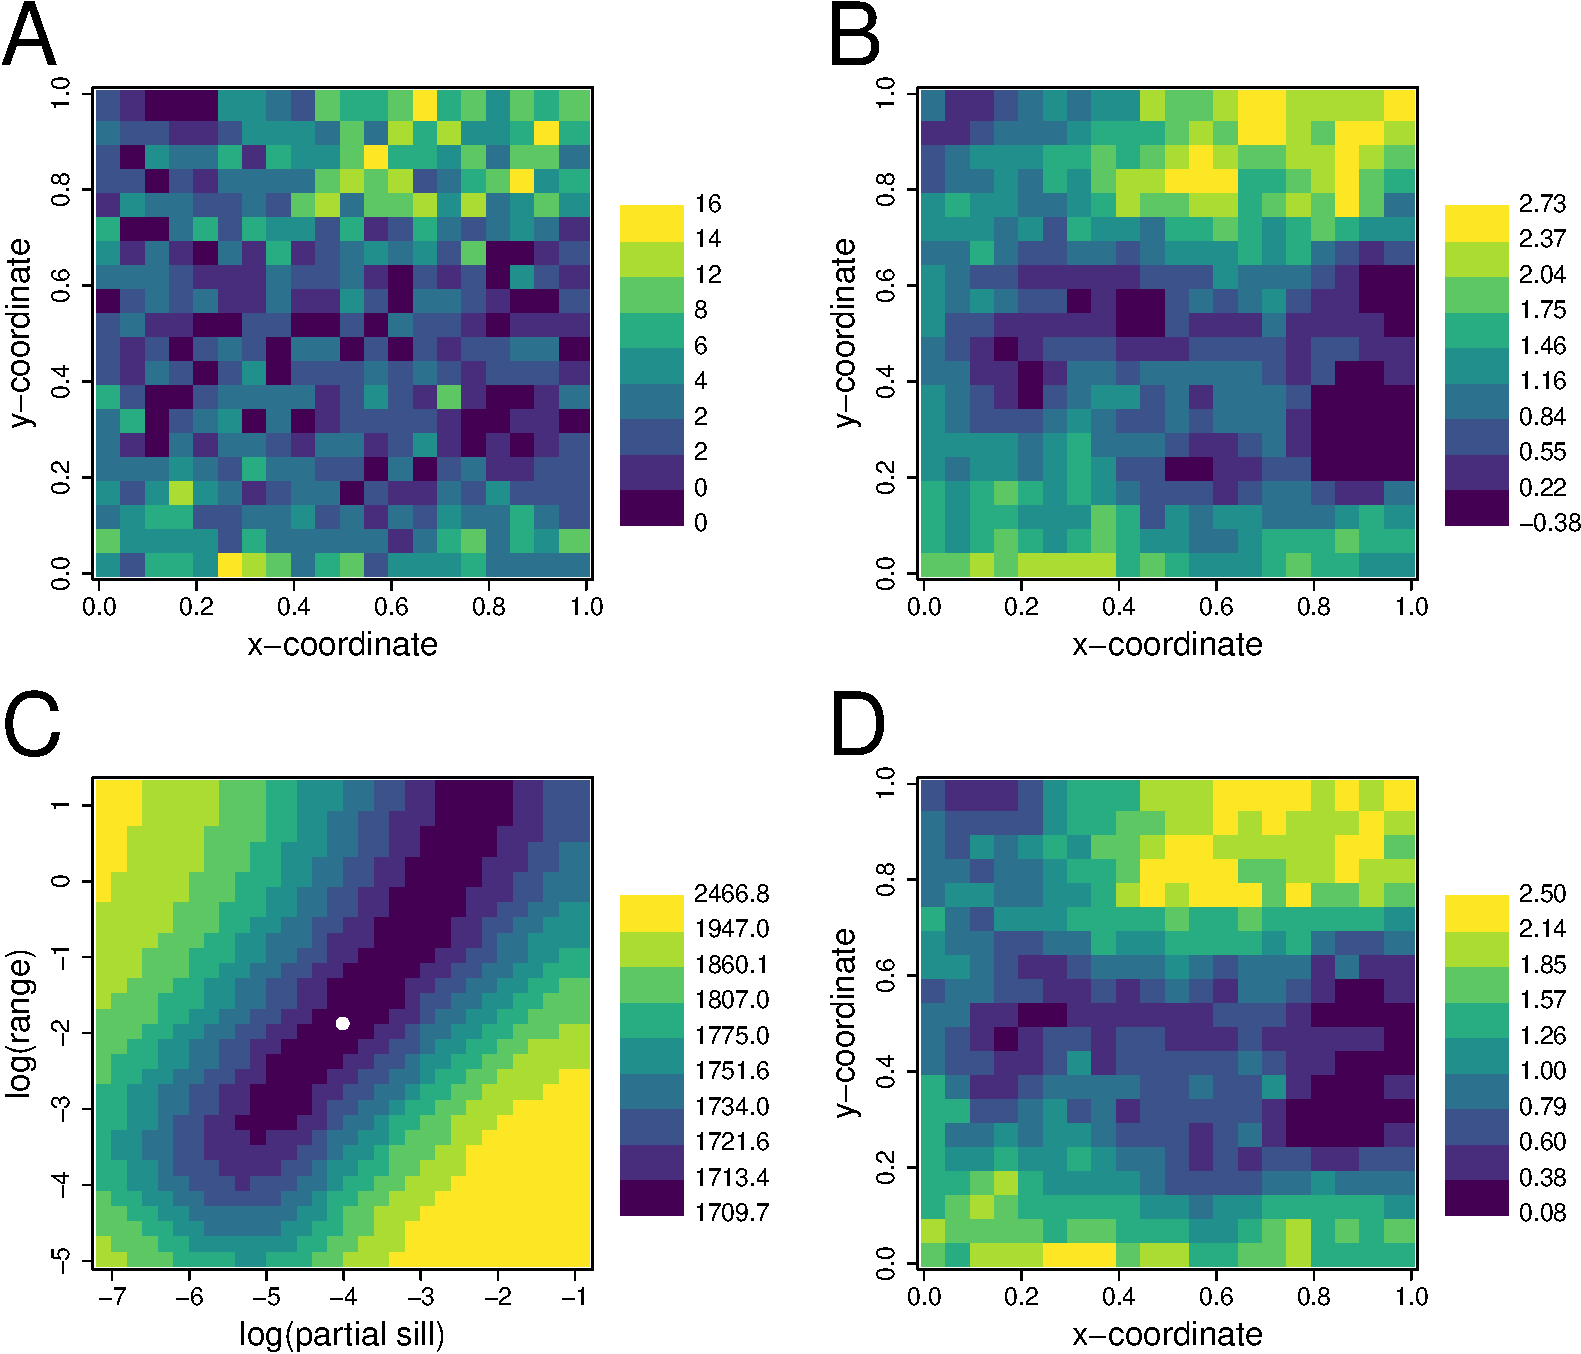
\includegraphics[width=.8\linewidth]{figures/pois_likelihood_estimation}
  \end{center}
  \caption{Estimation for simulated data. A. Simulated count data using the model described in the text.  B. The true simulated $\mathbf{w}$ values. C. The likelihood surface of the simulated data.  The white circle shows the estimated value.  D. The estimated $\hat{\mathbf{w}}$ values. \label{Fig:sglm_likelihood_estimation}}
\end{figure}

Of course, this is just one simulation.  How does it work on average?  Are the estimators and predictors unbiased, and are we estimating their variance correctly so that they have the proper confidence and prediction interval coverage?  In order to answer these questions, we did a computer simulation experiment.  Here, we created 200 locations randomly on the unit square. We used the same autocovariance model as above, $\cov(w(\mathbf{s}),w(\mathbf{s} + r)) = \exp(-r) + 0.0001\mathcal{I}(r = 0)$.  For the mean structure, we used
$$
\textrm{E}(w_{i}) = \beta_{0} + \beta_{1}x_{i} + \beta_{2}\tau_{i} + \beta_{3}(x{:}\tau)_{i}
$$
where $x_{i}$ were randomly simulated from $\textrm{N}(0,1)$, $\tau_{i}$ were randomly simulated bernoulli variables with probability $p = 0.5$, and $(x{:}\tau)_{i}$ was in interaction between the normally-distributed and bernoulli-distributed explanatory variables.  We set $\mathbf{\beta} = (0.5, 0.5, -0.5, 0.5)$.  We also created 100 prediction locations where we used a $10 \times 10$ square grid of equally-spaced prediction points throughout the unit square.  Explanatory variables were also simulated at the prediction locations, and so 300 $w_{i}$ values were simulated from $\textrm{N}(\mathbf{X}\boldsymbol{\beta},\boldsymbol{\Sigma}_{\boldsymbol{\theta}})$. We then created the observed data as counts from a Poisson distribution conditional on the $\mathbf{w}$, where at each spatial location we independently simulated the Poisson random variable with mean equal to $\exp(w_{i})$.  We simulated 2000 data sets to assess bias and confidence/prediction interval coverage.

For each simulated data set, we first estimated the covariance parameters using \eqref{eq:m2LLmargMLE}, using an exponential autocorrelation model as before. Then, we used the estimated covariance parameters as plugin values for the autocovariance model to obtain $\boldsymbol{\Sigma}_{\hat{\boldsymbol{\theta}}}$, and along with the estimated $\hat{\mathbf{w}}$, we estimated fixed effects $\hat{\boldsymbol{\beta}} = \mathbf{B}\hat{\mathbf{w}}$.  To estimate bias, we took the average of $\hat{\boldsymbol{\beta}} - \boldsymbol{\beta}$ over all 2000 simulated data sets. We also formed 90\% confidence intervals as $\hat{\boldsymbol{\beta}} \pm 1.645 \widehat{\textrm{se}}(\hat{\boldsymbol{\beta}})$, where $\widehat{\textrm{se}}(\hat{\boldsymbol{\beta}})$ were the square roots of the diagonal elements of \eqref{eq:sglmm_varfe}.  Over the 2000 simulations, we computed the proportion of times that the confidence interval contained the true value.  If we are estimating the variances of $\hat{\boldsymbol{\beta}}$ well, the coverage should be close to 90\%. We also computed the confidence interval coverage based on the naive unadjusted $\mathbf{C}_{\boldsymbol{\beta}}$. 

The results are shown in Table~\ref{tab:sglm_fe}, where we see that there is very little bias in estimating any of the parameters in $\boldsymbol{\beta}$.  The confidence interval coverage for $\beta_{0}$ is slightly low, but the confidence interval coverages for $\beta_{1}$ - $\beta_{3}$ are very close to 90\% when using \eqref{eq:sglmm_varfe}, but they are much too short when using $\mathbf{C}_{\boldsymbol{\beta}}$.

We also used the estimated covariance parameters in $\boldsymbol{\Sigma}_{\hat{\boldsymbol{\theta}}}$ and the estimated $\hat{\mathbf{w}}$ to make predictions at all 100 values for each simulated data set using $\hat{\mathbf{u}} = \boldsymbol{\Lambda}\hat{\mathbf{w}}$.  To estimate bias, we took the average of $\hat{\mathbf{u}} - \mathbf{u}$ for each simulated data set, where recall that $\mathbf{u}$ contains 100 simulated values, and then averaged those across the 2000 simulated data sets.  We also formed 90\% prediction intervals as $\hat{\mathbf{u}} \pm 1.645 \widehat{\textrm{se}}(\hat{\mathbf{u}})$, where $\widehat{\textrm{se}}(\hat{\mathbf{u}})$ were the square roots of the diagonal elements of \eqref{eq:sglmm_varpred}. Over the 2000 simulations, we computed the proportion of times that the prediction intervals contained the true values, which should be about 90\%. Table~\ref{tab:sglm_fe} gives the prediction results, which show little indication of bias, and coverage was very close to 90\%.

\begin{table}[H] 
	\caption{Bias and coverage for estimation of fixed effects $\boldsymbol{\beta}$ and for prediction of $\mathbf{u}$ at unobserved locations.  Coverage is for 90\% confidence and prediction intervals, and CI90$_{c}$ used the corrected versions in \eqref{eq:sglmm_varfe} and \eqref{eq:sglmm_varpred}, while CI90$_{u}$ shows coverage for the uncorrected standard-error estimator based on $\mathbf{C}_{\boldsymbol{\beta}}$ and the uncorrected prediction standard errors using (9.5).  \label{tab:sglm_fe}}
\begin{center}
\begin{tabular}{|c|rrr|}
\hline
\hline
effect & bias & CI90$_{u}$ & CI90$_{u}$ \\
\hline{}
$\beta_{0}$ & -0.006 & 0.865 & 0.875 \\ 
$\beta_{1}$ &    -0.003 & 0.360 & 0.905 \\ 
$\beta_{2}$ &   0.002 & 0.310 & 0.898 \\ 
$\beta_{3}$ &   -0.004 & 0.331 & 0.896 \\ 
$\hat{\mathbf{u}}$ &   0.034 & 0.692 & 0.894 \\  
\hline
\hline
\end{tabular}
\end{center}
\end{table}


%%%%%%%%%%%%%%%%%%%%%%%%%%%%%%%%%%%%%%%%%%%%%%%%%%%%%%%%%%%%%%%%%%%%%%%%%%%%%%%%
%%%%%%%%%%%%%%%%%%%%%%%%%%%%%%%%%%%%%%%%%%%%%%%%%%%%%%%%%%%%%%%%%%%%%%%%%%%%%%%%                BIBLIOGRAPHY
%%%%%%%%%%%%%%%%%%%%%%%%%%%%%%%%%%%%%%%%%%%%%%%%%%%%%%%%%%%%%%%%%%%%%%%%%%%%%%%%
%%%%%%%%%%%%%%%%%%%%%%%%%%%%%%%%%%%%%%%%%%%%%%%%%%%%%%%%%%%%%%%%%%%%%%%%%%%%%%%%

%\bibliographystyle{consbiol}
\bibliographystyle{/mnt/ExtraDrive1/Work/shTex/asa}
\bibliography{spglm.bib}
%\bibliographystyle{/home/jay/Data/shTex/shTex/asa}
%\bibliography{/home/jay/Data/shTex/shTex/StatBibTex.bib}




\end{document}

